% Monitoramento de servidores Linux por web sites.
%====================================================================================================
% TCC
%----------------------------------------------------------------------------------------------------
% Autor				    : Eduardo Balan
% Orientador		  : Kleber Krugrer
% Instituição 		: UFMS - Universidade Federal do Mato Grosso do Sul
% Departamento		: CPCX - Sistema de Informação
%----------------------------------------------------------------------------------------------------
% Data de criação	: 29 de Março de 2017
%====================================================================================================

\chapter{Desenvolvimento}\label{cap:Desenvolvimento}

Neste trabalho foi desenvolvido um sistema para monitoramento de servidores Linux, utilizando a arquitetura cliente-servidor. O sistema consiste em duas aplicações, um \textit{web service} desenvolvido em Java para o qual foi dado o nome de MonitorWeb-Api, e outra aplicação em C++, executada nos servidores Linux como cliente, tendo o nome de MonitorWeb-Cli.

O MonitorWeb-Cli realiza a leitura dos dados de seu hospedeiro, tais como CPU (\textit{Central Processing Unit}), memória, banco de dados e \textit{swap}. Esse procedimento é realizado de acordo com a configuração de tempo desejada pelo usuário. Para cada leitura realizada, o sistema realiza o envio dos dados para o MonitorWeb-Api. Ele também pode realizar rotinas de \textit{backups} (cópia de segurança) e \textit{vaccum} (processo de limpeza no banco de dados) do banco dados PostgreSQL, tanto no hospedeiro quanto em outro computador a qual tenha acesso pela rede. Após efetuar esses procedimentos, o MonitorWeb-Cli envia mensagens para o MonitorWeb-Api que por sua vez armazena essas informações.

Um MonitorWeb-Api é responsável por receber os dados de diversos MonitorWeb-Cli e realizar a persistência no banco de dados. Também é responsável por armazenar as configurações dos clientes, tais como o intervalo de envio dos dados de monitoramento e as informações dos procedimentos de \textit{backup}. Essas configurações são capturadas periodicamente conforme as configurações do usuário. A API também pode ser utilizada para disponibilizar os dados dos servidores para aplicações de \textit{frontend} (aplicações responsáveis por coletar a entrada do usuário e processá-la para adequá-la a uma especificação em que o back-end possa utilizar).

Na \autoref{Img:MonitorWeb-Api} e na \autoref{Img:MonitorWeb-Cli} se faz uma ilustração das principais tecnologias utilizadas na implementação da aplicação MonitorWeb-Api e MonitorWeb-Cli, respectivamente.

\begin{figure}[H]
	\centering
	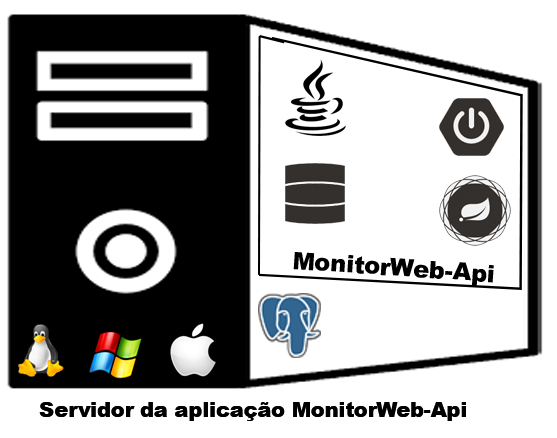
\includegraphics[width=0.5\textwidth]{figuras/MonitorWeb/monitorWeb-Api.jpg}
	\caption[Ilustração das tecnologias utilizadas no MonitorWeb-Api]{Ilustração das tecnologias utilizadas no MonitorWeb-Api. A aplicação pode ser executada nos sistemas operacionais Linux, Windows e MacOS. Esta aplicação foi desenvolvida em Java e utilizou o banco de dados PostgreSQL para a persistência dos dados. Os principais \textit{frameworks} utilizados foram: Spring Boot, Spring Framework, Spring Data}
	\label{Img:MonitorWeb-Api}
\end{figure}

\begin{figure}[H]
	\centering
	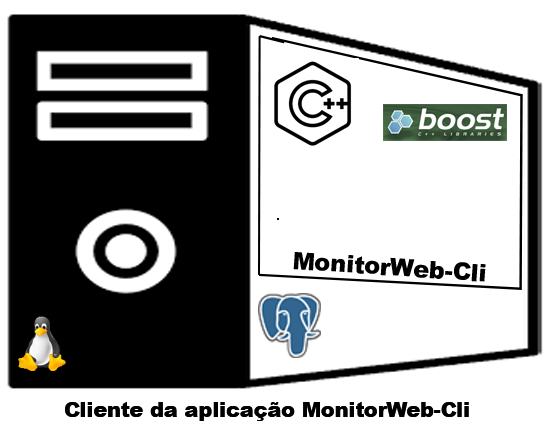
\includegraphics[width=0.5\textwidth]{figuras/MonitorWeb/monitorWeb-Cli.jpg}
	\caption[Ilustração das tecnologias utilizadas no MonitorWeb-Cli]{Ilustração das tecnologias utilizadas no MonitorWeb-Cli. A aplicação foi desenvolvida para o sistema operacional Linux utilizando a linguagem C++. Esta aplicação fez uso da biblioteca Boost para fazer requisições HTTP e permite a realização dos procedimentos de \textit{backup} e \textit{vacuum} em bancos de dados PostgreSQL.}
	\label{Img:MonitorWeb-Cli}
\end{figure}

\section{MonitorWeb-Api}\label{sec:MonitorWeb-Api}

O MonitorWeb-Api é um \textit{web service} desenvolvido utilizando a tecnologia Spring Boot para o desenvolvimento de uma aplicação ReST que utiliza o protocolo HTTP/1.1 na comunicação com sistemas clientes. Para enviar os dados entre as aplicações foi utilizado o JSON (\textit{JavaScript Object Notation}) em vez do XML por ter sua estrutura menor e consumir menos trafego na rede \cite{Saudate:2014}. Para a persistência dos dados foi utilizado o banco de dados PostgreSQL \cite{PostgreSQL:2017}.

Um MonitorWeb-Api possui a capacidade de trabalhar com diversos MonitorWeb-Cli simultaneamente, conforme exibido na \autoref{Img:CliApi}.

\begin{figure}[H]
	\centering
	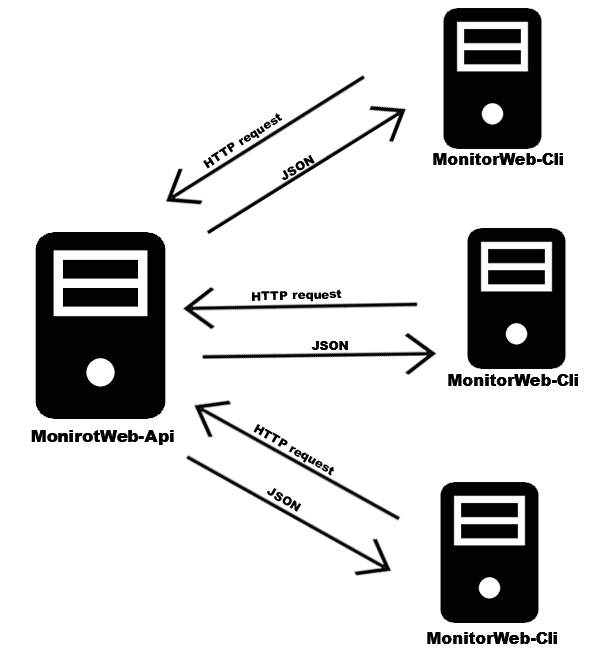
\includegraphics[width=0.7\textwidth]{figuras/MonitorWeb/MonitorWeb-CliComMonirotWeb-Api.jpg}
	\caption[Comunicação entre o MonitorWeb-Api e as aplicações MonitoresWeb-Cli]{Comunicação entre o MonitorWeb-Api e as aplicações MonitoresWeb-Cli. Um MonitorWeb-Api pode receber requisições de diversos MonitoresWeb-Cli, executando uma ação na base de dados e retornando uma resposta em formato JSON.}
	\label{Img:CliApi}
\end{figure}

Os atributos da classe Servidor, descritos na \autoref{Tab:VariaveisServidor} representa um MonitorWeb-Cli.

\begin{table}[!ht]
\centering
\begin{tabular}{|l|l|}
\hline
{\color[HTML]{000000} \textbf{Variáveis}} & {\color[HTML]{000000} \textbf{Descriçães}}                                                                \\ \hline
id                                     & \multicolumn{1}{p{13.00cm}|}{Número único para cada objeto do tipo Servidor. (Gerado Automaticamente) }\\ \hline
dominio                                & \multicolumn{1}{p{13.00cm}|}{A qual domínio o servidor pertence. (Não obrigatório). Esse atributo será tratado na \autoref{subsubsec:DiagramaClasseUsuarios}} \\ \hline
dthr\_cadastro                         & \multicolumn{1}{p{13.00cm}|}{Data e hora do cadastro. (Valor gerado automaticamente)} \\ \hline
nome                                   & \multicolumn{1}{p{13.00cm}|}{Nome que o usuário deseja dar ao servidor.}  \\ \hline
empresa                                & \multicolumn{1}{p{13.00cm}|}{Nome da empresa (Não obrigatório)} \\ \hline
observacao                             & \multicolumn{1}{p{13.00cm}|}{Alguma observação a fazer sobre o servidor (Não obrigatório)} \\ \hline
\end{tabular}
\caption[Variáveis da classe Servidor e suas descrições.]{Variáveis da classe Servidor e suas descrições.}
\label{Tab:VariaveisServidor}
\end{table}


\subsection{Diagrama de Classes}\label{subsec:DiagramaDeClasses}

Um diagrama de classe pode ser visto na \autoref{Img:DiagramaDeClass1}, em que é mostrado resumidamente o relacionamento da classe Servidor com as outras classes da aplicação. Esse diagrama está separado em três partes enumeradas, descritas a seguir.

\begin{itemize}
		\item \autoref{Img:DiagramaDeClass1}, Grupo 1. As classes desse grupo possuem o prefixo Servidor e correspondem às configurações da aplicação e as configurações de rotinas do banco de dados.
		\item \autoref{Img:DiagramaDeClass1}, Grupo 2. Classes desse grupo possuem o prefixo Informacoes. Estas, representam registros cadastrados automaticamente pela aplicação MonitorWeb-Cli e fazem referência às informações do \textit{hardware} (componentes físicos de um computador). Os registros dessas classes são armazenados apenas no momento de inicialização do sistema, pois os valores não podem ser alterados sem a reinicialização da máquina. Exemplos desses valores são o modelo do processador e a quantidade de memória física. A descrição de cada classe desse grupo pode ser vista no \autoref{App:ApendiceA}.
		%\item \autoref{Img:DiagramaDeClass1} grupo número 2 (classes desse grupo possuem o prefixo Informacoes) são classes que serão cadastradas automaticamente pela aplicação MonitorWeb-Cli e fazem referencia a os valores do servidor que são inseridos a cade vez que a aplicação é iniciada. Esses tipos de valores não tem como ser mudado sem que a maquina seja reiniciada. Um exemplos desse valor é o modelo do processador, ele nunca será mudado sem que a maquina seja reiniciada.
		\item \autoref{Img:DiagramaDeClass1}, Grupo 3. Classes desse grupo possuem o prefixo Monitoramento. Os objetos dessas classes representam registros gerados automaticamente pelo MonitorWeb-Cli com os valores de desempenho de \textit{hardware} e \textit{software} monitorados periodicamente. Exemplos dos valores armazenados por objetos dessas classes são: quantidade de memória e CPU que estão sendo utilizadas, situação dos procedimentos de \textit{backups}. A descrição de cada classe desse grupo pode ser vista no \autoref{App:ApendiceA}
		%\item \autoref{Img:DiagramaDeClass1} grupo número 3 (classes desse grupo possuem o prefixo Monitoramento) são classes que contem valores que precisam ser monitorados de tempos em tempo. Os intervalos de tempo do monitoramento das classe MonitoramentoCpu, MonitoramentoMemoria e MonitoramentoSwap são configurado através do objeto "ServidorConfig" como pode ser visto pela \autoref{Tab:VariaveisServidorConfig}. Exemplos dos valores armazenados por objetos dessa classe são quanto dememória está sendo utilizado e quantos Mhz cada núcleo do processador está utilizado.
\end{itemize}


\begin{figure}[H]
	\centering
	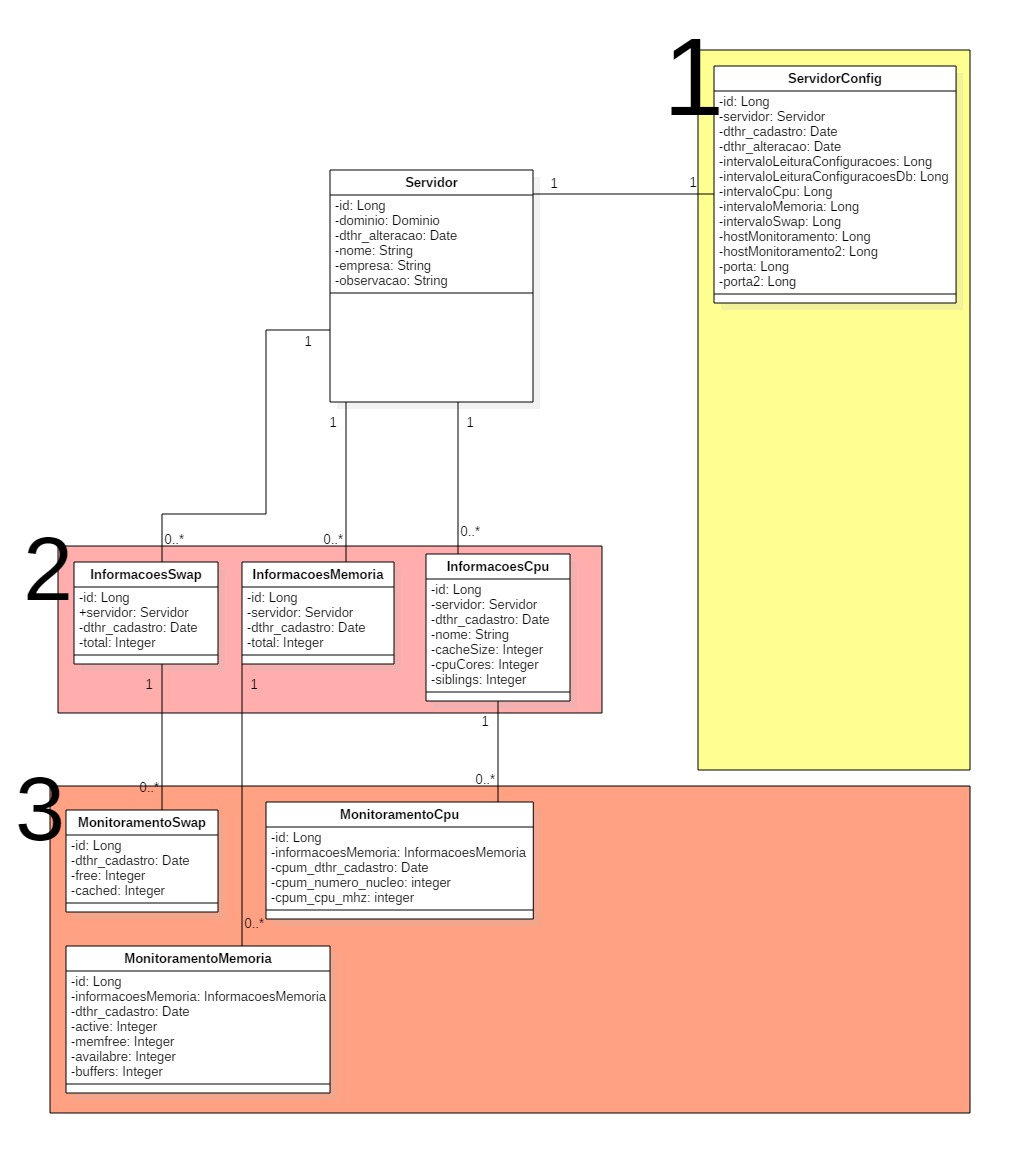
\includegraphics[width=1.0\textwidth]{figuras/DiagramaDeClass1.jpg}
	\caption[Diagrama de classe resumido 1.]{Diagrama de classe resumido 1, separados pelos grupos 1 à 3 que correspondem, respectivamente, às configurações que o usuário deve fazer, informações geradas pelo MonitorWeb-Cli e monitoramentos gerados pelo MonitorWeb-Cli}
	\label{Img:DiagramaDeClass1}
\end{figure}



\subsubsection{Classe ServidorConfig}
Como pode ser visto na \autoref{Img:DiagramaDeClass1}, a classe ServidorConfig possui um relacionamento de um-para-um com a classe Servidor, indicando assim que um objeto de Servidor pode ter somente um ServidorConfig. Essa classe é vital para o funcionamento do MonitorWeb-Cli. Dentro dela estão as configurações mínimas para que um MonitorWeb-Cli saiba como trabalhar. Na \autoref{Tab:VariaveisServidorConfig} explica-se detalhadamente a classe ServidorConfig.

Na \autoref{Tab:VariaveisServidorConfig}, o valor padrão das variáveis são apenas sugestões. O usuário pode alterar qualquer um deles, porém, é altamente recomendado que esses valores nunca sejam iguais a 0. Caso isso aconteça, o MonitorWeb-Cli enviará o máximo de informações que puder sem qualquer intervalo de tempo. Isso acaba consumindo o máximo de recurso (memória, cpu e disco) do sistema operacional hospedeiro.

\begin{table}[H]
\centering
\begin{tabular}{|l|l|}
\hline
{\color[HTML]{000000} \textbf{Variáveis}} & {\color[HTML]{000000} \textbf{Descriçães}} \\ \hline
id                                     & \multicolumn{1}{p{10.00cm}|}{Número único para cada objeto do tipo ServidorConfig. (Gerado Automaticamente)} \\ \hline
servidor                               & \multicolumn{1}{p{10.00cm}|}{Informa com qual servidor esse registro está relacionado.}
\\ \hline
dthr\_cadastro                         & \multicolumn{1}{p{10.00cm}|}{Data e hora do cadastro. (Gerado Automaticamente)}\\ \hline
dthr\_alteracao                        & \multicolumn{1}{p{10.00cm}|}{Data e hora que foi realizado a ultima alteração. (Gerado Automaticamente)(Essa funcionalidade não foi implementada)}\\ \hline
intervaloLeituraConfiguracoes          & \multicolumn{1}{p{10.00cm}|}{Intervalo em segundos para o MonitorWeb-Cli ler as configurações da classe ServidorConfig, e se reconfigurar(Valor padrão 120 s).} \\ \hline
intervaloLeituraConfiguracoesDb        & \multicolumn{1}{p{10.00cm}|}{Intervalo em segundos para o  MonitorWeb-Cli ler as configurações da classe ServidorConfigDb, e se reconfigurar(Valor padrão 120 s). Essa classe é mostrada na \autoref{subsubsec:ClasseServidorConfigDb}} \\ \hline
intervaloCpu                           & \multicolumn{1}{p{10.00cm}|}{Intervalo em segundos para o MonitorWeb-Cli enviar um registro da classe MonitoramentoCpu.(Valor padrão 1 s)}\\ \hline
intervaloMemoria                       & \multicolumn{1}{p{10.00cm}|}{Intervalo em segundos para o MonitorWeb-Cli enviar um registro da classe MonitoramentoMemoria.(Valor padrão 1 s)}\\ \hline
intervaloSwap                          & \multicolumn{1}{p{10.00cm}|}{Intervalo em segundos para o MonitorWeb-Cli enviar um registro da classe MonitoramentoSwap.(Valor padrão 1 s)} \\ \hline
hostMonitoramento                      & \multicolumn{1}{p{10.00cm}|}{IP que o MonitorWeb-Cli deve se comunicar.}\\ \hline
hostMonitoramento2                     & \multicolumn{1}{p{10.00cm}|}{IP secundário que o MonitorWeb-Cli deve se comunicar caso o servidor principal não esteja funcionando.(Essa funcionalidade não foi implementada)} \\ \hline
porta                                  & \multicolumn{1}{p{10.00cm}|}{Porta da aplicação para o MonitorWeb-Cli saber em que porta o MonitorWeb-Api está rodando.} \\ \hline
porta2                                 & \multicolumn{1}{p{10.00cm}|}{Porta da aplicação secundária para o MonitorWeb-Cli saber em que porta o MonitorWeb-Api está rodando.(Essa funcionalidade não foi implementada)} \\ \hline
\end{tabular}
\caption[Variáveis da classe ServidorConfig e suas descrições.]{Variáveis da classe ServidorConfig e suas descrições.}
\label{Tab:VariaveisServidorConfig}
\end{table}


\subsubsection{Classe ServidorConfigDb}\label{subsubsec:ClasseServidorConfigDb}

No diagrama de classe mostrado na \autoref{Img:DiagramaDeClass2} existem duas novas classes: a ServidorConfigDb no grupo um e a MonitoremantoPostgres no grupo três. Além das classes, um novo grupo número 4 é mostrado. Nesse grupo temos as \textit{enums} da aplicação, utilizadas em algumas classes.

\begin{figure}[H]
	\centering
	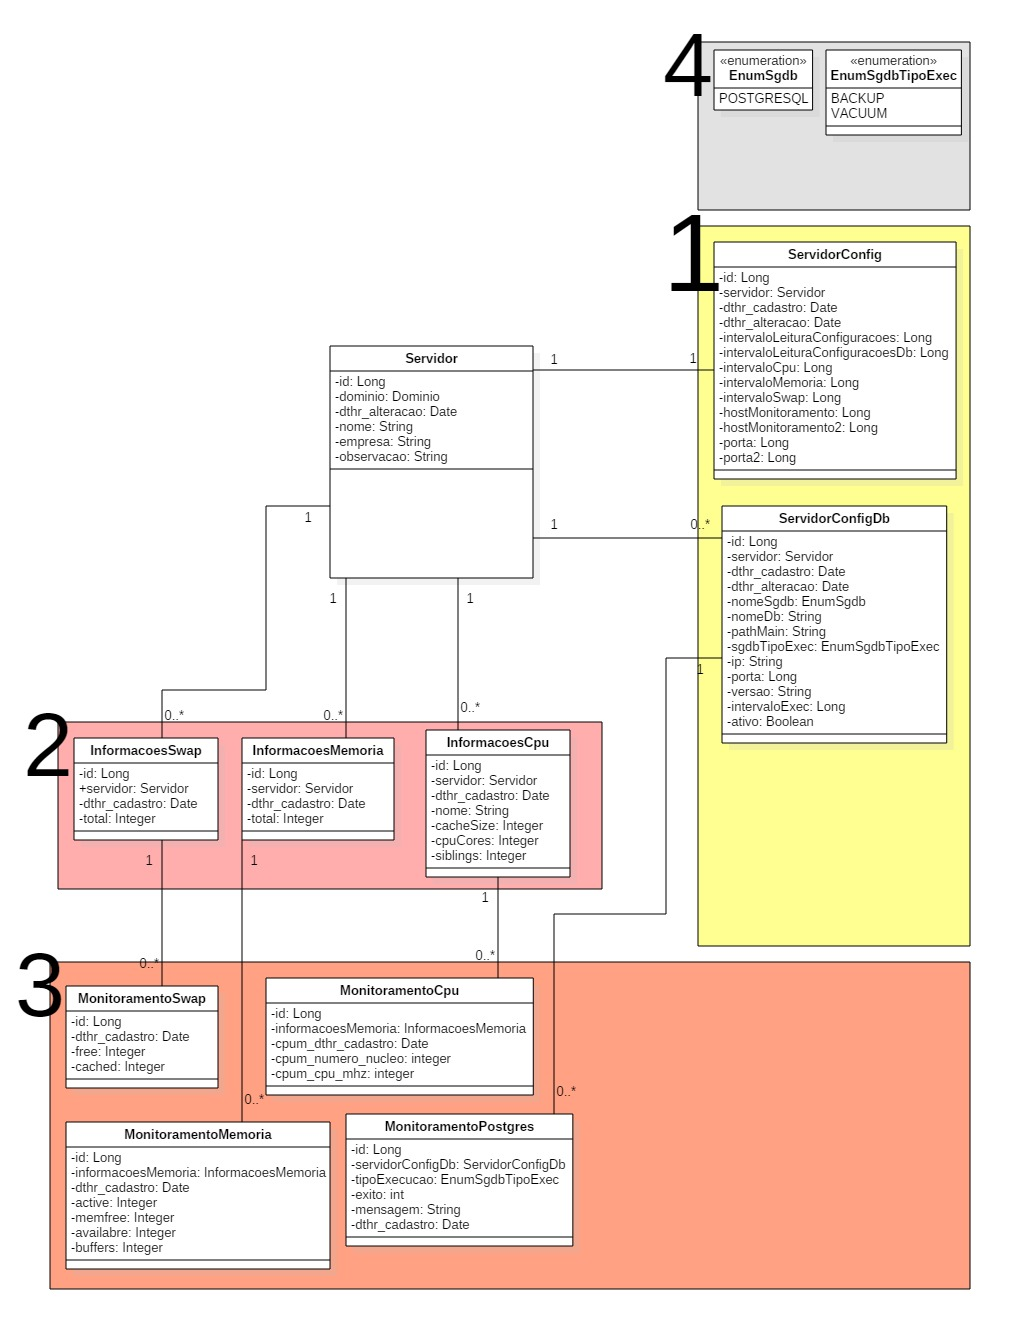
\includegraphics[width=1.0\textwidth]{figuras/DiagramaDeClass2.jpg}
	\caption[Diagrama de classe resumido 2.]{Diagrama de classe resumido 2, separados pelos grupos 1 à 4 que correspondem, respectivamente, às configurações que o usuário deve fazer, informações geradas pelo MonitorWeb-Cli, monitoramentos gerados pelo MonitorWeb-Cli e \textit{enums} da aplicação.}
	\label{Img:DiagramaDeClass2}
\end{figure}

A classe ServidorConfigDb é responsável por criar rotinas de \textit{backup} e \textit{vacuum} para o MonitoreWeb-Cli executar. Essa classe possui um relacionamento de muitos-para-um com a classe Servidor, o que indica que em um servidor pode ter diversas rotinas de \textit{backup} e \textit{vacuum}. Na \autoref{Tab:VariaveisServidorConfigDb} é explicada de forma minuciosa a classe ServidorConfigDb.

Essa classe também pode ser utilizada para o MonitoreWeb-Cli executar o procedimento de \textit{backup} e \textit{vacuum} em outro computador, para isso basta ser informado o IP da máquina que se deseja executar o procedimento e que a maquina esteja habilitada para fazer esse procedimento pela rede.

A classe MonitoremantoPostgres é responsável por armazenar os resultados dos \textit{backups} e dos procedimentos de \textit{vacuum} da classe ServidorConfigDb. A descrição de cada variável dessas classe pode ser vista no \autoref{App:ApendiceA}.

\begin{table}[H]
\centering
\begin{tabular}{|l|l|}
\hline
{\color[HTML]{000000} \textbf{Variável}} & {\color[HTML]{000000} \textbf{Descrição}}\\ \hline
id                                       & \multicolumn{1}{p{12.50cm}|}{Número único para cada objeto do tipo ServidorConfigDb. (Gerado Automaticamente) }\\ \hline
servidor                                 & \multicolumn{1}{p{12.50cm}|}{Indica com qual objeto Servidor esse registro está relacionado.}\\ \hline
dthr\_cadastro                           & \multicolumn{1}{p{12.50cm}|}{Data e hora do cadastro. (Gerado Automaticamente) } \\ \hline
dthr\_alteracao                          & \multicolumn{1}{p{12.50cm}|}{Data e hora que foi realizado a ultima alteração. (Gerado Automaticamente)}\\ \hline
nomeSgdb                                 & \multicolumn{1}{p{12.50cm}|}{É uma enum do tipo EnumSgdb, que informa em qual SGDB o procedimento será executado. Atualmente somente o postgreSQL é suportado. }\\ \hline
nomeDb                                   & \multicolumn{1}{p{12.50cm}|}{Nome do banco de dados que o procedimento será executado.}\\ \hline
pathMain                                 & \multicolumn{1}{p{12.50cm}|}{Caminho para as libs que executam o backup.}\\ \hline
sgdbTipoExec                             & \multicolumn{1}{p{12.50cm}|}{É uma enum do tipo EnumSgdbTipoExec o qual informa se o procedimento é um backup ou um vacuum.} \\ \hline
ip                                       & \multicolumn{1}{p{12.50cm}|}{IP para onde devera ser executado o procedimento. }\\ \hline
porta                                    & \multicolumn{1}{p{12.50cm}|}{Porta que será executado o procedimento. }\\ \hline
versao                                   & \multicolumn{1}{p{12.50cm}|}{Versão do SGDB.}\\ \hline
intervaloExec                            & \multicolumn{1}{p{12.50cm}|}{Intervalo de tempo que o MonitoreWeb-Cli deve executar esse procedimento.}\\ \hline
ativo                                    & \multicolumn{1}{p{12.50cm}|}{Controle para ativar e desativar o procedimento.}\\ \hline
\end{tabular}
\caption[Variáveis da classe ServidorConfigDb e suas descrições.]{Variáveis da classe ServidorConfigDb e suas descrições.}
\label{Tab:VariaveisServidorConfigDb}
\end{table}

\subsubsection{Classe ServidorConfigInformacoesDb}

No diagrama de classe mostrado na \autoref{Img:DiagramaDeClass3} existem duas novas classes: a ServidorConfigInformacoesDb no Grupo 1 e a MonitoremantoPostgresInformacoes no Grupo 3.

\begin{figure}[H]
	\centering
	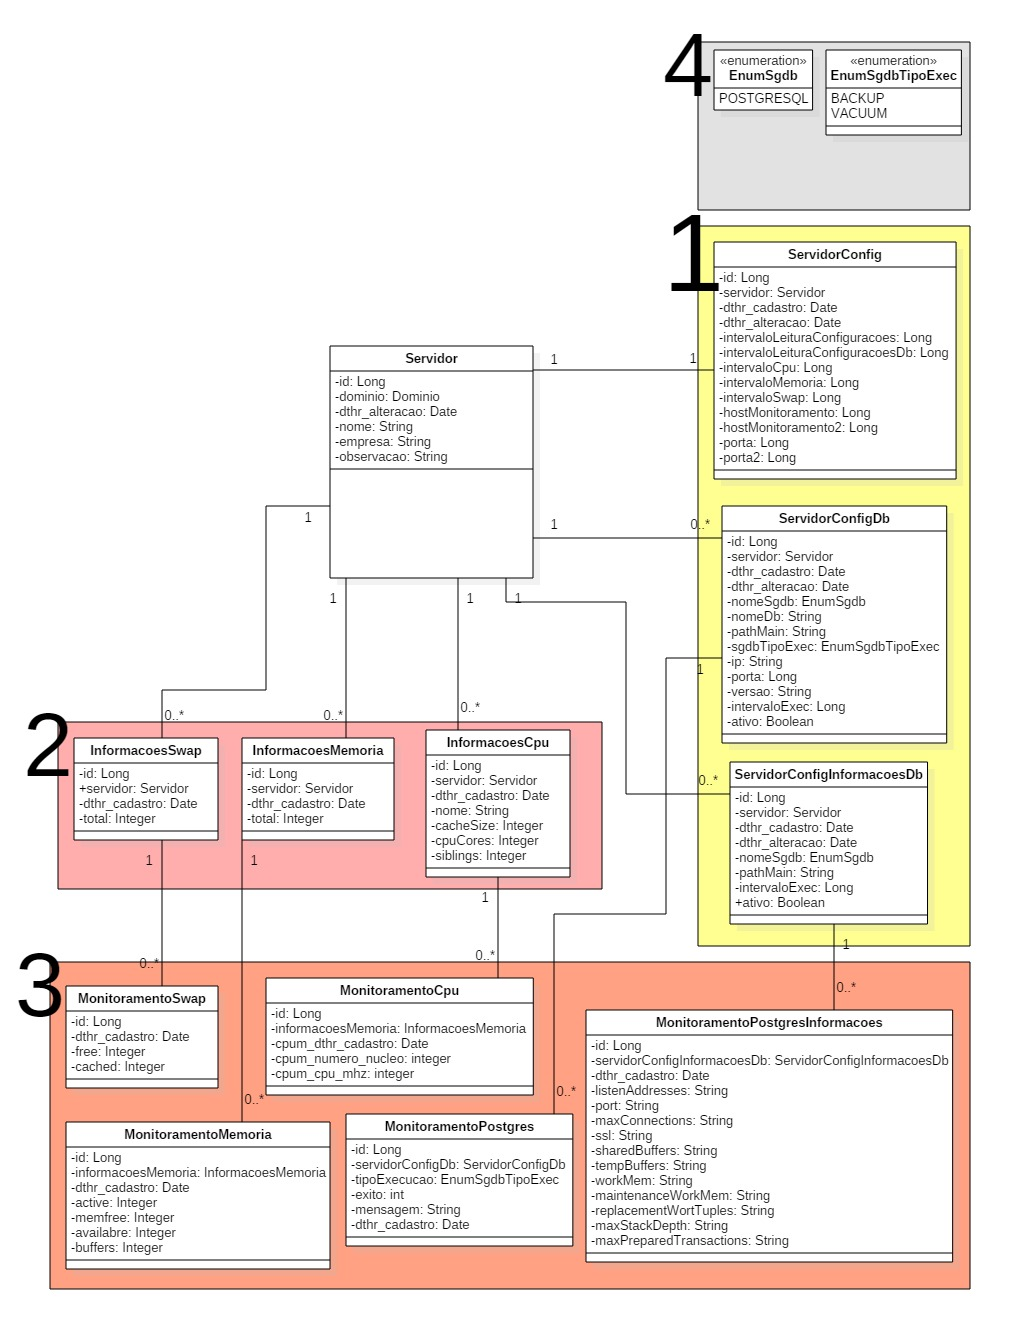
\includegraphics[width=1.0\textwidth]{figuras/DiagramaDeClass3.jpg}
	\caption[Diagrama de classe resumido 3.]{Diagrama de classe resumido 3, separados pelos grupos 1 à 4 que correspondem respectivamente a configurações que o usuário deve fazer, informações geradas pelo MonitorWeb-Cli, monitoramentos gerados pelo MonitorWeb-Cli e enums da aplicação.}
	\label{Img:DiagramaDeClass3}
\end{figure}

 A classe ServidorConfigInformacoesDb é responsável por criar uma rotina para ler o arquivo com as configurações principais do postgreSQL (postgresql.conf). Essa classe possui um relacionamento de muitos-para-um com a classe Servidor, uma vez que o servidor pode ter várias versões do banco de dados. Na \autoref{Tab:VariaveisServidorConfigInformacoesDb} descreve-se detalhadamente a classe ServidorConfigInformacoesDb.

A classe MonitoremantoPostgres é responsável por armazenar os resultados da classe ServidorConfigInformacoesDb. A descrição de cada variável da classe MonitoremantoPostgres pode ser vista no \autoref{App:ApendiceA}.


\begin{table}[H]
\centering
\begin{tabular}{|l|l|}
\hline
{\color[HTML]{000000} \textbf{Variável}} & {\color[HTML]{000000} \textbf{Descrição}}\\ \hline
id                                       & \multicolumn{1}{p{12.50cm}|}{Número único para cada objeto do tipo ServidorConfigDb. (Gerado Automaticamente)} \\ \hline
servidor                                 & \multicolumn{1}{p{12.50cm}|}{Indica com qual objeto Servidor esse registro está relacionado. }\\ \hline
dthr\_cadastro                           & \multicolumn{1}{p{12.50cm}|}{Data e hora do cadastro. (Gerado Automaticamente)}\\ \hline
dthr\_alteracao                          & \multicolumn{1}{p{12.50cm}|}{Data e hora que foi realizado a ultima alteração. (Gerado Automaticamente)}\\ \hline
nomeSgdb                                 & \multicolumn{1}{p{12.50cm}|}{É uma enum do tipo EnumSgdb, que informa em qual SGDB o procedimento será executado. Atualmente somente o postgreSQL é suportado. } \\ \hline
pathMain                                 & \multicolumn{1}{p{12.50cm}|}{Caminho para o arquivo postgresql.conf . }\\ \hline
intervaloExec                            & \multicolumn{1}{p{12.50cm}|}{Intervalo de tempo que o MonitoreWeb-Cli deve executar esse procedimento.} \\ \hline
ativo                                    & \multicolumn{1}{p{12.50cm}|}{Controle para ativar e desativar o procedimento. }\\ \hline
\end{tabular}
\caption[Variáveis da classe ServidorConfigInformacoesDb e suas descrições.]{Variáveis da classe ServidorConfigInformacoesDb e suas descrições.}
\label{Tab:VariaveisServidorConfigInformacoesDb}
\end{table}



\subsubsection{Diagrama de classe Usuários}\label{subsubsec:DiagramaClasseUsuarios}

No diagrama de classe mostrado na \autoref{Img:DiagramaDeClass4} existe um Grupo 5. Esse grupo está relacionado a um cadastro de usuário. Ele não é utilizado pelo MonitorWeb-Cli mas pode ser utilizado por implementações futuras para uma aplicação \textit{frontend} para o sistema. 

No Grupo 5 existem duas classes: a Usuario, que corresponde ao cadastro de contas de usuário na aplicação, e a Dominio, que corresponde a uma classe para dividir os usuários por grupo. Dessa forma, uma empresa que tenha diversos setores pode separar mais facilmente qual usuário tem acesso a qual grupo de servidores.

Além das duas classes, existe a classe UsuarioHasDominio que é simplesmente uma classe para uma ligação de muitos-para-muitos entre as classes Usuario e Dominio. A descrição de cada variável da classe Usuario e Dominio pode ser vistas no \autoref{App:ApendiceA}.
 
\begin{figure}[H]
	\centering
	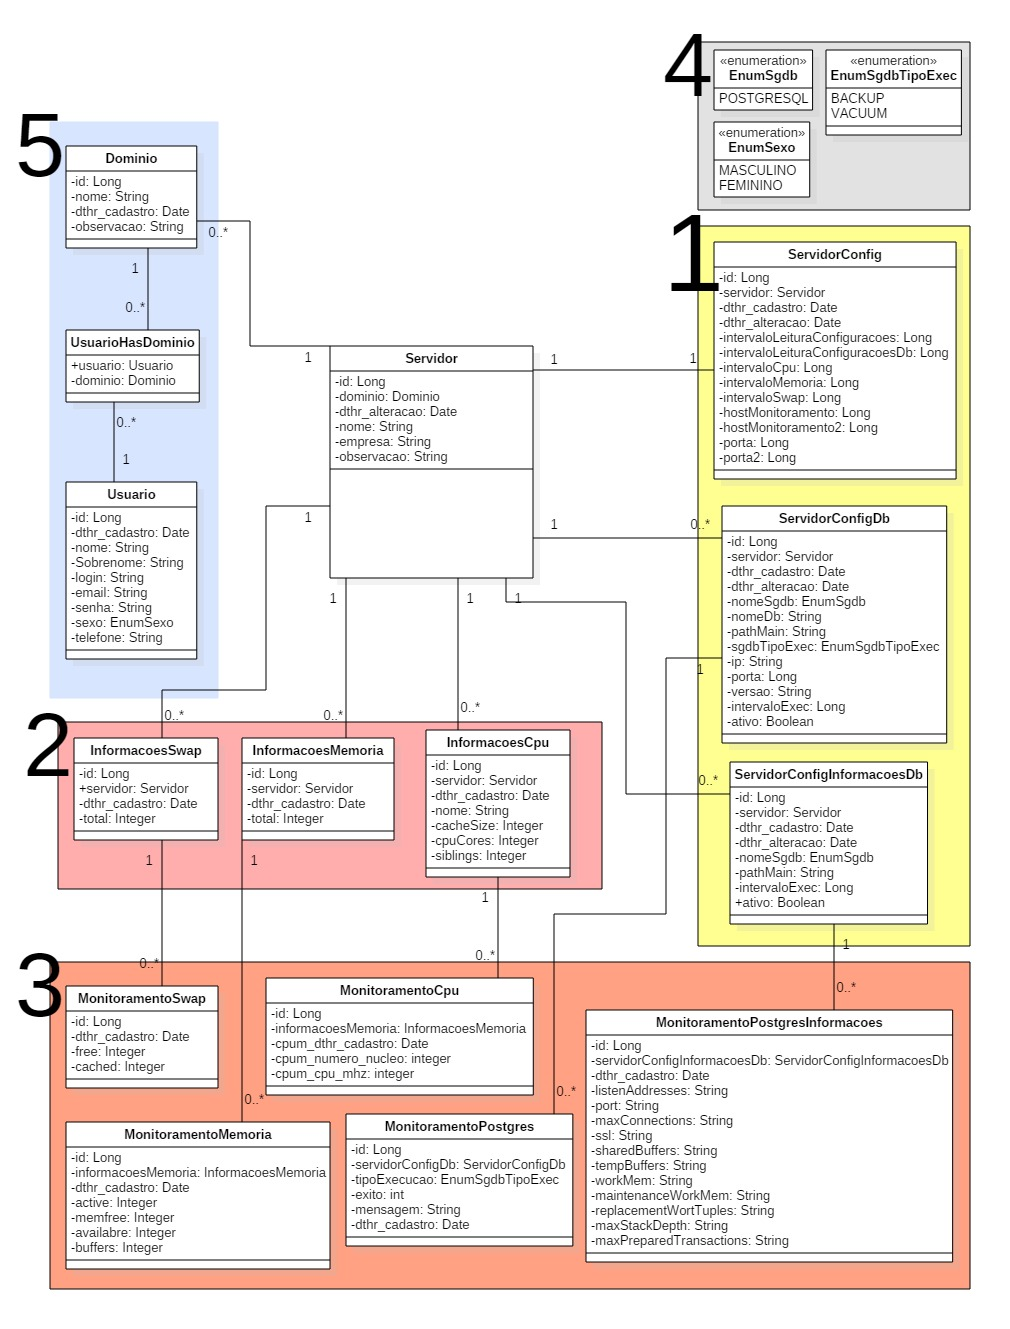
\includegraphics[width=1.0\textwidth]{figuras/DiagramaDeClass4.jpg}
	\caption[Diagrama de classe resumido 4.]{Diagrama de classe resumido 4, separados pelos grupos 1 à 5 que correspondem respectivamente a configurações que o usuário deve fazer, informações geradas pelo MonitorWeb-Cli, monitoramentos gerados pelo MonitorWeb-Cli, enums da aplicação e cadastro de usuários.}
	\label{Img:DiagramaDeClass4}
\end{figure}


\subsubsection{Diagrama de classe Completo}

No diagrama de classe mostrado na \autoref{Img:DiagramaDeClass} existe uma nova classe abstrata chamada de GenericEntity, sendo essa a superclasse para todas as entidades do sistema. A sua função é implementar os métodos \textit{equals} e \textit{hashCode} da classe Object. EXPLICAR O PORQUE!!! Além disso, ela cria os métodos abstratos getId, setId, getDthr\_cadastro e setDthr\_cadastro obrigando todos os métodos que estenderem dela a implementa-los.

A classe GenericEntity recebe um tipo T genérico que estende de Serializable. Esse tipo T representa o tipo da variável id da entidade, para que a aplicação saiba como gerar determinados métodos. A classe GenericEntity pode ser vista no \autoref{App:ApendiceB}.



\begin{figure}[H]
	\centering
	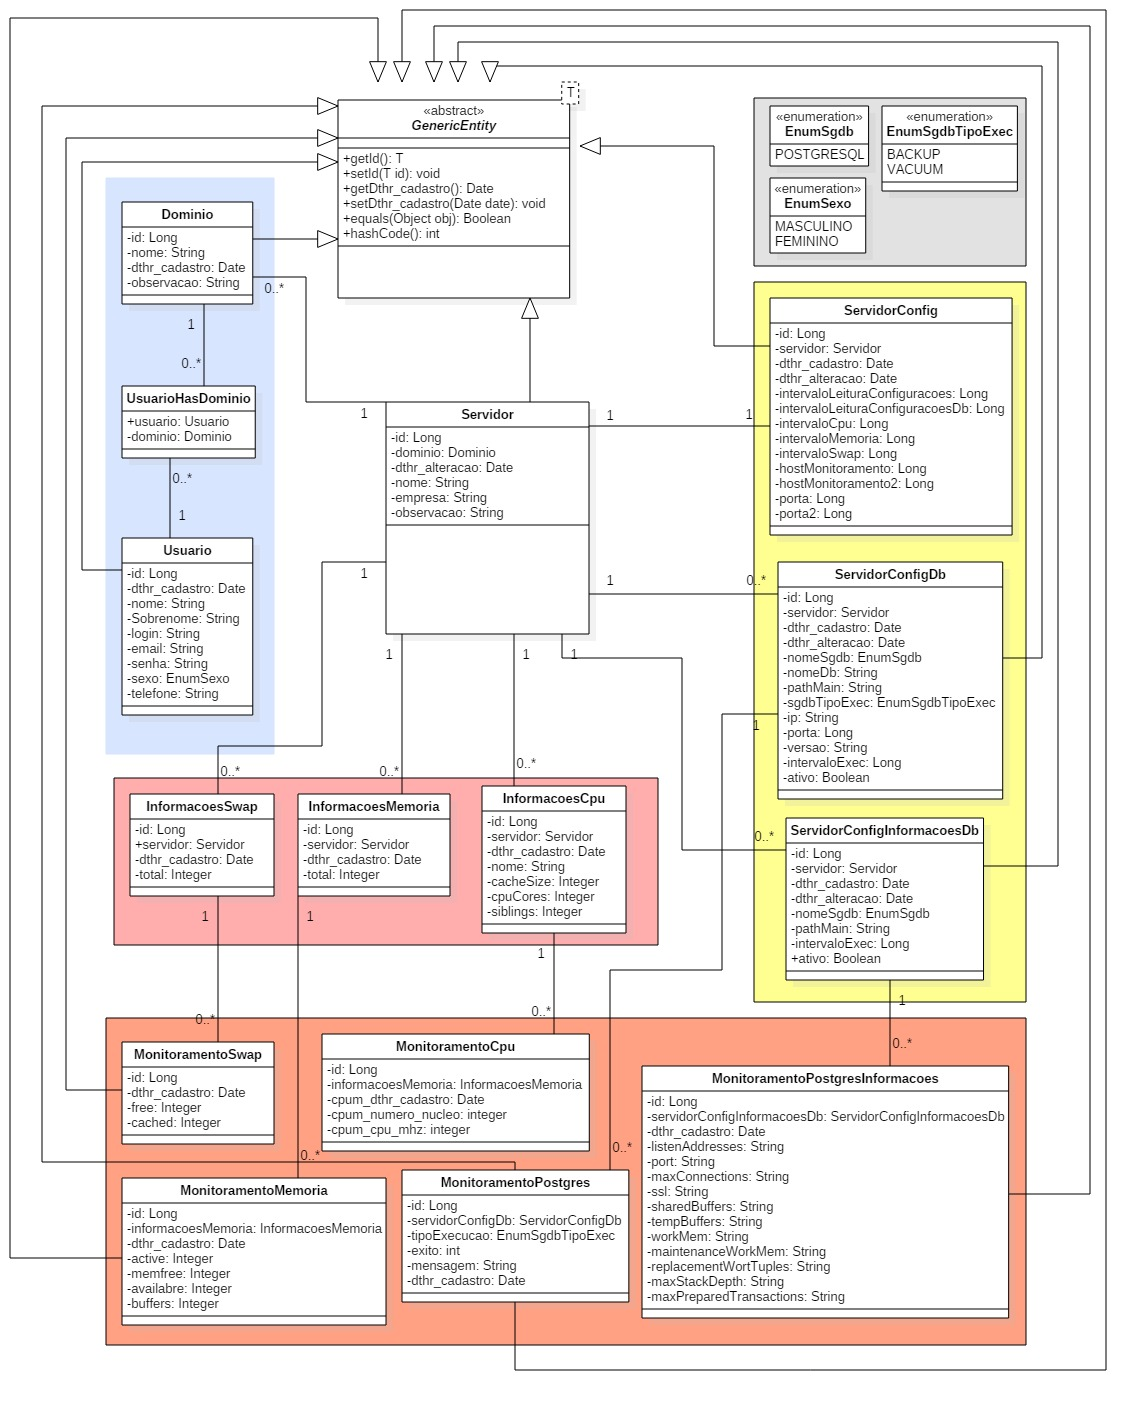
\includegraphics[width=1.0\textwidth]{figuras/DiagramaDeClass.jpg}
	\caption[Diagrama de classe completo.]{Diagrama de classe completo, separados pelos grupos 1 à 5 que correspondem respectivamente a configurações que o usuário deve fazer, informações geradas pelo MonitorWeb-Cli, monitoramentos gerados pelo MonitorWeb-Cli, enums da aplicação e cadastro de usuários.}
	\label{Img:DiagramaDeClass}
\end{figure}

\subsection{Configurações Apache Maven}\label{subsec:ConfiguraçõesApacheMaven}

Como visto na \autoref{sec:ApacheMaven} o Apache Maven é um gerenciador de pacotes responsável por gerir as dependências por meio do arquivo POM.
Esse arquivo é localizado na raiz do projeto (\url{/pom.xml}) e pode ser conferido no \autoref{App:ApendiceB}.

A seguir estão as principais dependências do projeto MonitorWeb-Api.

\begin{itemize}\label{List:Pom}
		\item \autoref{Func:POMMonitorWebApi}, linha 3 - spring-boot-starter-parent. Dependência do Spring Boot. Está dependência define uma versão base para que não seja necessário especificar as versões nos outros pacotes do Spring \cite{springBoot:2017}.
		
		\item \autoref{Func:POMMonitorWebApi}, linha 10 - spring-boot-starter-data-jpa. Dependência do Spring Data Jpa. Traz todas as dependências da JPA necessárias para o mapeamento das entidades \cite{springDataJpa:2017}.
		
		\item \autoref{Func:POMMonitorWebApi}, linha 15 - spring-boot-starter-web. Essa dependência identifica que a aplicação terá uma arquitetura \textit{web}, executando de forma embutida o servidor tomcat \cite{springBoot:2017}.
		
		\item \autoref{Func:POMMonitorWebApi}, linha 20 - spring-boot-starter-logging. Dependência responsável pelo registro de log automático \cite{springBoot:2017}.
		
		\item \autoref{Func:POMMonitorWebApi}, linha 25 - spring-boot-starter-test. Dependência do Spring Boot com bibliotecas de teste unitário, incluindo JUnit, Hamcrest e Mockito \cite{springBoot:2017}.
		
		\item \autoref{Func:POMMonitorWebApi}, linha 31 - postgresql, Dependência que fornece um conjunto padrão de interfaces para bancos de dados compatíveis com SQL \cite{PostgreSQL:2017}.
	
\end{itemize}


\subsection{Configurações Spring Boot}\label{subsec:ConfiguraçõesApplicationProperties}

O Spring Boot fornece um arquivo de configuração com o nome de application.properties, e pode ser encontrado na pacote \url{/src/main/resources}. Dentro desse arquivo pode ser feitas configurações de acordo com a necessidade do projeto \cite{springBoot:2017}. No \autoref{Func:applicationProperties} encontra-se o application.properties do MonitoreWeb-Api e a seguir uma lista contendo a descrição de cada configuração.

\begin{itemize}
		\item \autoref{Func:applicationProperties}, linha 2: server.port - Porta em que a aplicação será executada \cite{springBoot:2017}.
		
		\item \autoref{Func:applicationProperties}, linha 5: spring.jackson.date-format - Formato em que a data será apresentada \cite{springBoot:2017}.
		
		\item \autoref{Func:applicationProperties}, linha 10: logging.path - Indica o local do arquivo de \textit{log} \cite{springBoot:2017}.
		
		\item \autoref{Func:applicationProperties}, linha 19: spring.datasource.url - URL de conexão para o banco de dados \cite{springBoot:2017}.
		
		\item \autoref{Func:applicationProperties}, linha 20: spring.datasource.username - Usuario do banco de dados \cite{springBoot:2017}.
		
		\item \autoref{Func:applicationProperties}, linha 21: spring.datasource.password - Senha do banco de dados \cite{springBoot:2017}.
		
		\item \autoref{Func:applicationProperties}, linha 22: spring.jpa.database-platform - Vários bancos de dados têm mais de um dialeto e essa propriedade especifica qual o hibernate irá utilizar \cite{springBoot:2017}.
		
		\item \autoref{Func:applicationProperties}, linha 23: spring.datasource.driverClassName - Classe do \textit{driver} que será utilizado para conexão \cite{springBoot:2017}.
		
\end{itemize}

\begin{lstlisting}[style=LIVRE, label=Func:applicationProperties,caption={[Arquivo application.properties com as principais configurações do projeto.]Arquivo application.properties com as principais configurações do projeto.}]
## Portas
server.port=8081

## Formatador de datas do jackson
spring.jackson.date-format= yyyy-MM-dd'T'HH:mm:ss.SSSZ

## --------------------------------------------------------------------
## POSTGRES
## --------------------------------------------------------------------
spring.datasource.url=jdbc:postgresql://localhost/webmonitor
spring.datasource.username=postgres
spring.datasource.password=postgres
spring.jpa.database-platform=org.hibernate.dialect.PostgreSQLDialect
spring.datasource.driverClassName=org.postgresql.Driver

\end{lstlisting}


\subsection{Estrutura do Projeto}\label{subsec:EstruturaDoProjeto}

O projeto é dividido em seis pacotes Java que podem ser vistos na \autoref{Img:estruturaDePastaPojeto}, e uma classe na raiz com nome WebMonitorApp, a qual é responsável por iniciar a aplicação. Na \autoref{Tab:DescricaoDasPastasProjeto} apresenta-se a descrição de cada pacote.

\begin{figure}[H]
	\centering
	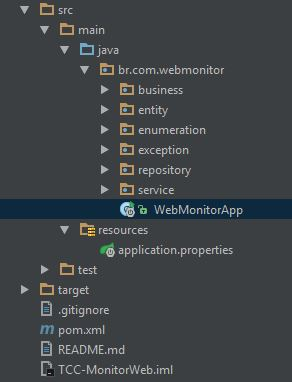
\includegraphics[width=0.5\textwidth]{figuras/estruturaPojeto.JPG}
	\caption[Estrutura dos pacotes Java do projeto.]{Estrutura dos pacotes Java do projeto.}
	\label{Img:estruturaDePastaPojeto}
\end{figure}
	

\begin{table}[!ht]
\centering
\begin{tabular}{|l|l|}
\hline
\multicolumn{1}{|c|}{{\color[HTML]{000000} \textbf{Pasta}}} & {\color[HTML]{000000} \textbf{Descrição}} \\ \hline
business                                                    & \multicolumn{1}{p{10.00cm}|}{Responsável pelas regras de negocio. \autoref{subsubsec:business}. }\\ \hline
entity                                                      & \multicolumn{1}{p{10.00cm}|}{Contém as entidades do sistema. \autoref{subsec:DiagramaDeClasses}. }\\ \hline
enumeration                                                 & \multicolumn{1}{p{10.00cm}|}{Contém as enum da aplicação.}\\ \hline
exception                                                   & \multicolumn{1}{p{10.00cm}|}{Contém as exception da aplicação.}\\ \hline
repository                                                  & \multicolumn{1}{p{10.00cm}|}{Interfaces para gerar os acessos ao banco de dados. \autoref{subsubsec:Repository}.}\\ \hline
service                                                     & \multicolumn{1}{p{10.00cm}|}{Responsáveis pelos serviços da aplicação. \autoref{subsubsec:Service}.}\\ \hline
\end{tabular}
\caption{Descrição das pacotes do projeto.}
\label{Tab:DescricaoDasPastasProjeto}
\end{table}


\subsubsection{Repository}\label{subsubsec:Repository}



O pacote repository Contém as interfaces de acesso ao banco de dados que são controladas pelo Spring Data. Todas essas interfaces devem herdar JpaRepository. Dessa forma, os métodos de consulta e persistência são gerados automaticamente pelo Spring Data.

Na \autoref{Img:estruturaDePastaRepository} pode ser visto que cada entidade da aplicação possui uma interface repository. O padrão de nomenclatura utilizado nas interfaces é: <nome-da-entidade> seguido pela palavra "Repository".

\begin{figure}[H]
	\centering
	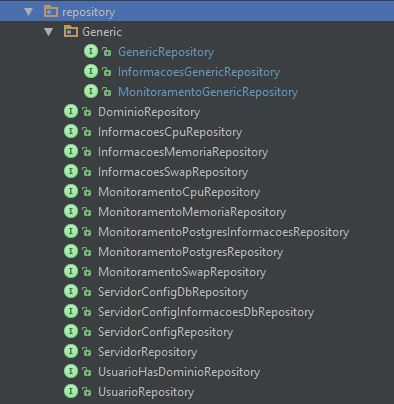
\includegraphics[width=0.5\textwidth]{figuras/estruturaPojetoRepository.JPG}
	\caption[Pacote Repository.]{Pacote Repository.}
	\label{Img:estruturaDePastaRepository}
\end{figure}


\subsubsection{Business}\label{subsubsec:business}

O pacote business é responsável pelas regras de negocio da aplicação. Cada entidade contém uma classe business correspondente que segue o padrão de nomenclatura: <nome-da-entidade> mais "BO", como pode ser visto na \autoref{Img:estruturaDePastaBusiness}. 

Todas as classes da business herdam a classe GenericBO que Contém os métodos genéricos de inserção e exclusão do banco de dados. 

A GenericBO recebe dois parâmetros: o primeiro, um tipo genérico Entity que deve ser herdado da classe GenericEntity; o segundo, uma classe Repository que tenha implementado a interface JpaRepository para a respectiva entidade, o que informa que essa classe possui um repositório de acesso ao banco de dados controlado pelo Spring Boot. A classe GenericBO pode ser vista no \autoref{App:ApendiceB}.

\begin{figure}[H]
	\centering
	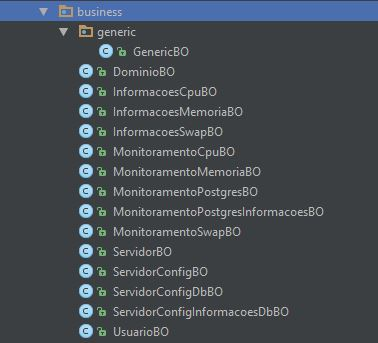
\includegraphics[width=0.5\textwidth]{figuras/estruturaPojetoBusines.JPG}
	\caption[Pacote Business.]{Pacote Business.}
	\label{Img:estruturaDePastaBusiness}
\end{figure}



\subsubsection{Service}\label{subsubsec:Service}

As classes do pacote service são as responsáveis por receber as requisições HTTP e responde-las de acordo com a especificação da arquitetura ReST. Cada entidade da aplicação contém uma classe Service correspondente que segue o padrão de nomenclatura: <nome-da-entidade> seguido da palavra "Service", como pode ser visto na \autoref{Img:estruturaDePastaService}.

Cada classe possui uma URL destinada a gerenciar seus recursos. Essas URLs aceitam os métodos GET, POST e DELETE que correspondem, respectivamente, à listagem, inserção e remoção de um objeto do recurso. Na \autoref{Tab:UrlRecursos} mostra-se essas URLs, e na \autoref{subsec:ConsumindoRecursos} está explicado como utiliza-las.


Na \autoref{Tab:UrlRecursos} os valores entre chaves representam o id do recurso à esquerda. Por exemplo, na URL \url{/usuario/7} está sendo feita uma requisição do recurso Usuario que tenha o id 7, e na URL \url{/servidor/11/informacoescpu} está sendo feita uma requisição do recurso InformaçõesCpu do servidor que tenha o id 11.

\begin{figure}[H]
	\centering
	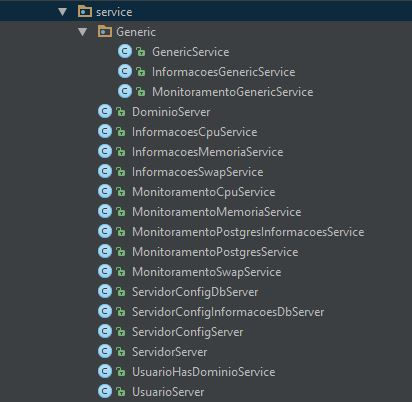
\includegraphics[width=0.5\textwidth]{figuras/estruturaPojetoService.JPG}
	\caption[Pacote Service.]{Pacote Service.}
	\label{Img:estruturaDePastaService}
\end{figure}


\begin{table}[H]
\centering
\begin{tabular}{|l|l|}
\hline
{\color[HTML]{000000} \textbf{Classe}}  & {\color[HTML]{000000} \textbf{URL}} \\ \hline
Usuario                           & \multicolumn{1}{p{9.00cm}|}{\url{/usuario }} \\ \hline
Dominio                           & \multicolumn{1}{p{9.00cm}|}{\url{/dominio }}  \\ \hline
Servidor                          & \multicolumn{1}{p{9.00cm}|}{\url{/servidor }}  \\ \hline
InformacoesCpu                   & \multicolumn{1}{p{9.00cm}|}{\url{/servidor/{idServidor}/informacoescpu}}   \\ \hline
InformacoesMemoria               & \multicolumn{1}{p{9.00cm}|}{\url{/servidor/{idServidor}/informacoesmemoria}}  \\ \hline
InformacoesSwap                  & \multicolumn{1}{p{9.00cm}|}{\url{/servidor/{idServidor}/informacoesswap }} \\ \hline
MonitoramentoCpu                 & \multicolumn{1}{p{9.00cm}|}{\url{/servidor/informacoes/{idInformacoesCpu}/monitoramentocpu}}\\ \hline
MonitoramentoMemoria             & \multicolumn{1}{p{9.00cm}|}{\url{/servidor/informacoes/{idInformacoesMemoria}/monitoramentomemoria}}\\ \hline
MonitoramentoPostgresInformacoes & \multicolumn{1}{p{9.00cm}|}{\url{/servidor/informacoes/{idInformacoesPostgresInformacoes}/monitoramentopostgresinformacoes}}\\ \hline
MonitoramentoPostgres            & \multicolumn{1}{p{9.00cm}|}{\url{/servidor/informacoes/{idInformacoesPostgres}/monitoramentopostgres}} \\ \hline
MonitoramentoSwap                & \multicolumn{1}{p{9.00cm}|}{\url{/servidor/informacoes/{idInformacoesSwap}/monitoramentoswap }}  \\  \hline
ServidorConfigDb                 & \multicolumn{1}{p{9.00cm}|}{\url{/servidor/{idServidor}/servidorconfiguracoesdb }}\\ \hline
ServidorConfigInformacoesDb      & \multicolumn{1}{p{9.00cm}|}{\url{/servidor/{idServidor}/servidorconfiguracoesinformacoesdb }}  \\  \hline
ServidorConfig                   & \multicolumn{1}{p{9.00cm}|}{\url{/servidor/{idServidor}/servidorconfiguracoes }}\\ \hline
\end{tabular}
\caption[URLs da aplicação MonitorWeb-Api.]{URLs da aplicação MonitorWeb-Api. }
\label{Tab:UrlRecursos}
\end{table}


\subsection{Consumindo Recursos do MonitorWeb-Api}\label{subsec:ConsumindoRecursos}

Os recursos do MonitorWeb-Api são consumidos utilizando o protocolo HTTP e seguindo o padrão ReST. Os métodos GET, PUT e DELETE servem, respectivamente, para consultar, inserir e excluir elementos na base de dados.

\subsubsection{GET}
O método GET pode ser utilizado de duas formas: a primeira traz um vetor com todos os objetos do recurso. Na URL \url{/servidor}, por exemplo, é retornado um vetor no formato \textit{json} contendo todos os objetos Servidor, conforme exibido no \autoref{Func:ConsumindoRecursosGet1}. A segunda forma é solicitar por um objeto específico mediante a um id. Como exemplo, na URL \url{/servidor/2}, a API retorna apenas o servidor cujo id é igual a 2 (\autoref{Func:ConsumindoRecursosGet2}).

\begin{lstlisting}[label=Func:ConsumindoRecursosGet1,caption={[Exemplo do vetor de resposta à solicitação GET para URL \url{/servidor}.]Exemplo do vetor de resposta à solicitação GET para URL \url{/servidor}.}]
[
    {
        "id": 1,
        "dominio": {
            "id": 1
        },
        "dthr_cadastro": "2017-01-02T03:11:18.075+0000",
        "nome": "Nome do Servidor 1",
        "empresa": "Empresa 1",
        "observacao": "OBS 1"
    },
    {
        "id": 2,
        "dominio": {
            "id": 2
        },
        "dthr_cadastro": "2017-01-03T03:01:59.099+0000",
        "nome": "Nome do Servidor 2",
        "empresa": "Empresa 2",
        "observacao": "OBS 2"
    }
]    
\end{lstlisting}





\begin{lstlisting}[label=Func:ConsumindoRecursosGet2,caption={[Exemplo do objeto de resposta a solicitação GET para URL \url{/servidor/2}.]Exemplo do objeto de resposta a solicitação GET para URL \url{/servidor/2}.}]
{
    "id": 2,
    "dominio": {
        "id": 2
    },
    "dthr_cadastro": "2017-01-03T03:01:59.099+0000",
    "nome": "Nome do Servidor 2",
    "empresa": "Empresa 2",
    "observacao": "OBS 2"
}
\end{lstlisting}

\subsubsection{POST}

O método POST é utilizado para inserir um novo objeto a um recurso. Por exemplo, para inserir um novo servidor no sistema, uma requisição POST deve ser realizada para a URL \url{/servidor} passando o objeto desejado, conforme mostra-se no \autoref{Func:ConsumindoRecursosPost1}. A resposta desta requisição é vista no \autoref{Func:ConsumindoRecursosPost2}.


\begin{lstlisting}[label=Func:ConsumindoRecursosPost1,caption={[Exemplo de uma requisição POST]Exemplo de uma requisição POST onde é passado o objeto que deseja ser inserido.]
POST /servidor HTTP/1.1
Host: 127.0.0.1:8081
Accept: application/json
{
    "dominio": {
        "id": 3
    },
    "nome": "Nome do Servidor 3",
    "empresa": "Empresa 3",
    "observacao": "OBS 3"
}
\end{lstlisting}

\begin{lstlisting}[label=Func:ConsumindoRecursosPost2,caption={[Exemplo de uma resposta a uma requisição POST] Exemplo de uma resposta a uma requisição POST}]
HTTP/1.1 200 OK
Content-Type: application/json
Content-Length: 197
{
    "id": 3,
    "dominio": {
        "id": 3
    },
    "dthr_cadastro": "2017-01-03T03:45:29.099+0000",
    "nome": "Nome do Servidor 3",
    "empresa": "Empresa 3",
    "observacao": "OBS 3"
}
\end{lstlisting}

\subsubsection{DELETE}

Uma requisição de DELETE é utilizada para remover um recurso da aplicação. Por exemplo, caso seja desejado remover o objeto de id 1, uma requisição utilizando-se o método DELETE para o recurso \url{/servidor/1} é enviada. Entretanto, utilizar esse método não garante a exclusão do recurso, uma vez que é necessário verificar a consistência do banco de dados. Caso o elemento a ser removido tenha relacionamento com outros objetos, o banco de dados impede sua remoção.

%# # # # # # # # # # # # # # # # # # # # # # # # # # # # # # # # # # # # # # # # # # # # # # # # # # # # # # # # # # # # # # # # # # # # # # # # # # # # # # # # # # # # # # # # # # # # # # # # # # # # # # # # # # # # # # # # # # # # # # # # # # # # # # # # # # # # # # # # # # # # # # # # # # # # # # # # # # # # # # # # # # # # # # # # # # # # # # # # # # # # # # # # # # # # # # # # # # # # # # # # # # # # # # # # # # # # # # # # # # # # # # # # # # # # # # # # # # # # # # # # # # # # # # # # # # # # # # # # # # # # # # # # # # # # # # # # # # # # # # # # # # # # # # # # # # # # # # # # # # # # # # # # # # # # # # # # # # # # # # # # # # # # # # # # # # # # # # # # # # # # # # # # # # # # # # # # # # # # # # # # # # # # # # # # # # # # # # # # # # # # # # # # # # # # # # # # # # # # # # # # # # # # # # # # # # # # # # # # # # # # # # # # # # # # # # # # # # # # # # # # # # # # # # # # # # # # # # # # # # # # # # # # # # # # # # # # # # # # # # # # # # # # # # # # # # # # # # # # # 


\section{MonitorWeb-Cli}\label{sec:MonitorWeb-Cli}

O MonitorWeb-Cli é um sistema cliente desenvolvido para executar em servidores Linux, de forma que todos os servidores monitorados executem uma única instância dessa aplicação. Esse sistema foi implementado utilizando-se a linguagem C++, porque tem como objetivo ler as informações e monitorar o desempenho do hardware, tais o desempenho de CPU e memórias, e enviar essas informações mediante a comunicação com um servidor ReST, utilizando-se o protocolo HTTP/1.1. Cada MonitorWeb-Cli possui a capacidade de enviar informações para um único MonitorWeb-Api.

\subsection{Configurações MonitorWeb-Cli}\label{subsubsec:ConfiguracesMonitorWeb-Cli}

O MonitorWeb-Cli possui dois arquivos de configurações: o ConfigLog.conf e o  ConfigFile.conf que devem estar no mesmo diretório do executável da aplicação.

\subsubsection{ConfigLog.conf}\label{subsubsec:ConfiguracesMonitorWeb-CliConfiglog}

O arquivo de configurações ConfigLog.conf é responsável por ativar e desativar os níveis de log da aplicação. Ele também gera um arquivo de log com nome de log.log que fica no mesmo diretório da aplicação. A \autoref{Tab:DescricaoArquivoConfiglog.conf} mostra os valores do arquivo ConfigLog.conf e suas descrições. No \autoref{Func:ExemploArquivoConfiglog.conf} é mostrado um e exemplo do arquivo ConfigLog.conf.

\begin{table}[H]
\centering
\begin{tabular}{|l|l|}
\hline
{\color[HTML]{000000} \textbf{Variável}} & {\color[HTML]{000000} \textbf{Valor}}                                                                \\ \hline
ativarEmTelaInfo                         & \multicolumn{1}{p{11.00cm}|}{Valor true ou false. Ativa ou desativa o log do tipo informações que é mostrado na tela do usuário.} \\ \hline
ativarEmTelaWarning                      & \multicolumn{1}{p{11.00cm}|}{Valor true ou false. Ativa ou desativa o log do tipo warning que é mostrado na tela do usuário.} \\ \hline
ativarEmTelaErro                         & \multicolumn{1}{p{11.00cm}|}{Valor true ou false. Ativa ou desativa o log do tipo erro que é mostrado na tela do usuário.}\\ \hline
ativarEmArquivoInfo                      & \multicolumn{1}{p{11.00cm}|}{Valor true ou false. Ativa ou desativa o log do tipo informações no arquivo log.log.}\\ \hline
ativarEmArquivoWarning                   & \multicolumn{1}{p{11.00cm}|}{Valor true ou false. Ativa ou desativa o log do tipo warning no arquivo log.log.}\\ \hline
ativarEmArquivoErro                      & \multicolumn{1}{p{11.00cm}|}{Valor true ou false. Ativa ou desativa o log do tipo erro no arquivo log.log.}\\ \hline
\end{tabular}
\caption[Descrição do arquivo ConfigLog.conf.]{Descrição de cada variável do arquivo ConfigLog.conf.}
\label{Tab:DescricaoArquivoConfiglog.conf}
\end{table}

\begin{lstlisting}[label=Func:ExemploArquivoConfiglog.conf,caption={[Exemplo de um arquivo ConfigLog.conf]Exemplo de um arquivo ConfigLog.conf}]
ativarEmTelaInfo:false
ativarEmTelaWarning:true
ativarEmTelaErro:true

ativarEmArquivoInfo:false
ativarEmArquivoWarning:true
ativarEmArquivoErro:true
\end{lstlisting}

\subsubsection{ConfigFile.conf}\label{subsec:ConfiguracesMonitorWeb-CliConfigFile}

O arquivo de configurações ConfigFile.conf é responsável pelas configurações da aplicação e sempre deve estar definido para a aplicação iniciar. Esse arquivo possui uma estrutura "chave e valor", com os mesmos atributos da classe ServidorConfig. Um exemplo pode ser visto no \autoref{Func:ExemploArquivoConfigFile.conf}. Quando o MonitoreWeb-Cli está em execução, esse arquivo é atualizado constantemente com a classe ServidorConfig do MonitorWeb-Api. Dessa forma, por meio do sistema servidor o usuário pode fazer dinamicamente alterações no sistema cliente. A \autoref{Tab:VariaveisArquivoConfigFile} mostra os valores do arquivo ConfigFile.conf e suas descrições.



\begin{table}[H]
\centering
\begin{tabular}{|l|l|}
\hline
{\color[HTML]{000000} \textbf{Variáveis}} & {\color[HTML]{000000} \textbf{Descriçães}} \\ \hline
id                                     & \multicolumn{1}{p{10.00cm}|}{Id do objeto de ServidorConfig correspondente a essa configuração.} \\ \hline
servidorid                             & \multicolumn{1}{p{10.00cm}|}{Informa com qual servidor esse registro está relacionado.}
\\ \hline
intervaloLeituraConfiguracoes          & \multicolumn{1}{p{10.00cm}|}{Intervalo em segundos para o MonitorWeb-Cli ler as configurações da classe ServidorConfig, e se reconfigurar(Valor padrão 120 s).} \\ \hline
intervaloLeituraConfiguracoesDb        & \multicolumn{1}{p{10.00cm}|}{Intervalo em segundos para o  MonitorWeb-Cli ler as configurações da classe ServidorConfigDb, e se reconfigurar(Valor padrão 120 s). Essa classe é mostrada na \autoref{subsubsec:ClasseServidorConfigDb}} \\ \hline
intervaloCpu                           & \multicolumn{1}{p{10.00cm}|}{Intervalo em segundos para o MonitorWeb-Cli enviar um registro da classe MonitoramentoCpu.(Valor padrão 1 s)}\\ \hline
intervaloMemoria                       & \multicolumn{1}{p{10.00cm}|}{Intervalo em segundos para o MonitorWeb-Cli enviar um registro da classe MonitoramentoMemoria.(Valor padrão 1 s)}\\ \hline
intervaloSwap                          & \multicolumn{1}{p{10.00cm}|}{Intervalo em segundos para o MonitorWeb-Cli enviar um registro da classe MonitoramentoSwap.(Valor padrão 1 s)} \\ \hline
hostMonitoramento                      & \multicolumn{1}{p{10.00cm}|}{IP que o MonitorWeb-Cli deve se comunicar.}\\ \hline
hostMonitoramento2                     & \multicolumn{1}{p{10.00cm}|}{IP secundário que o MonitorWeb-Cli deve se comunicar caso o servidor principal não esteja funcionando.(Essa funcionalidade não foi implementada)} \\ \hline
porta                                  & \multicolumn{1}{p{10.00cm}|}{Porta da aplicação para o MonitorWeb-Cli saber em que porta o MonitorWeb-Api está rodando.} \\ \hline
porta2                                 & \multicolumn{1}{p{10.00cm}|}{Porta da aplicação secundária para o MonitorWeb-Cli saber em que porta o MonitorWeb-Api está rodando.(Essa funcionalidade não foi implementada)} \\ \hline
\end{tabular}
\caption[Descrição do arquivo ConfigFile.conf.]{Descrição do arquivo ConfigFile.conf.}
\label{Tab:VariaveisArquivoConfigFile}
\end{table}

\begin{lstlisting}[label=Func:ExemploArquivoConfigFile.conf,caption={[Exemplo de um arquivo configFile.conf]Exemplo de um arquivo configFile.conf}]
id:1
servidorid:1
intervaloCpu:1
intervaloLeituraConfiguracoes:120
intervaloLeituraConfiguracoesDb:12
intervaloMemoria:1
intervaloSwap:1
hostMonitoramento:192.168.1.147
hostMonitoramento2:192.168.1.147
porta:8081
porta2:8081
\end{lstlisting}


\subsection{Diagrama de Classes}\label{subsec:DiagramaDeClassesMonitorwebcli}

Um diagrama de classe pode ser visto na \autoref{Img:Cli-Diagrama}, em que é mostrado os relacionamentos das classes no sistema MonitoreWeb-Cli. Neste, a classe principal é a ServidorConfig, pois todas as outras necessitam de um objeto da referida classe, contendo as configurações de comunicação com o MonitorWeb-Api. 

As classes das entidades do sistema MonitoreWeb-Cli apresentam os mesmos atributos das classes de entidade de MonitorWeb-Api, exceto que não há variáveis de controle de data (dthr\_cadastro e dthr\_alteracao), uma vez que esses dados são geradas pelo servidor. Ademais, possuem os seguintes atributos e métodos:

\begin{itemize}
	\item Métodos toJson: converte as variáveis do objeto em um JSON correspondente.
	
	\item Métodos fromJson: cria um objeto a partir de uma string em formato JSON.
	
	\item Métodos salvarConfiguracoesLocais: pertence a classe servidorConfig e é utilizado para salvar os valores do objeto no arquivo configFile.conf. 
	
	\item Métodos ler<nome-da-classe>:realizam a leitura das informações estáticas do hardware (aquelas que não são alteradas conforme a execução dos programas) da máquina hospedeira. Exemplo, a classe InformacoesCpu possui um método chamado "lerInformacoesCpu". Este, ao ser executado obtém as informações físicas da CPU, tais como o nome, o numero de \textit{cores} (núcleos), o tamanho da \textit{cache}, entre outras.
	
	\item Métodos monitorar<nome-da-classe>: esses métodos são responsáveis por enviar uma requisição POST para o MonitoreWeb-Api contendo as informações de monitoramento (dinâmicas) do hardware, tais como a taxa de uso da CPU ou a quantidade de memória física utilizada.
	
	\item Métodos sincronizarConfigLocalComApi: realiza uma requisição para o servidor ReST pedindo os dados das configurações atuais. Assim que as solicitações são recebidas, este método atualiza as configurações locais da máquina hospedeira. Este método é importante porque o usuário pode, em tempo real, modificar as configurações para, por exemplo, alterar o intervalo entre os monitoramentos. Por esse motivo, as aplicações cliente precisam verificar periodicamente (em intervalo também configurável) essas mudanças.
    
    \item Métodos threadSincronizarConfigLocalComApi: esses métodos criam uma \textit{thread} para ficar executando o método sincronizarConfigLocalComApi, independente do resto da aplicação.
    
    \item Métodos threadMonitorar<Nome-da-classe>:esses métodos criam uma \textit{thread} para ficar executando o método monitorar<nome-da-classe> independente do resto da aplicação.
    
    \item Variável *thread: toda classe possível de criar uma \textit{thread} de monitoramento possui este ponteiro, assim é possível interromper e remover a \textit{thread} quando o objeto é removido.
\end{itemize}



\begin{figure}[H]
	\centering
	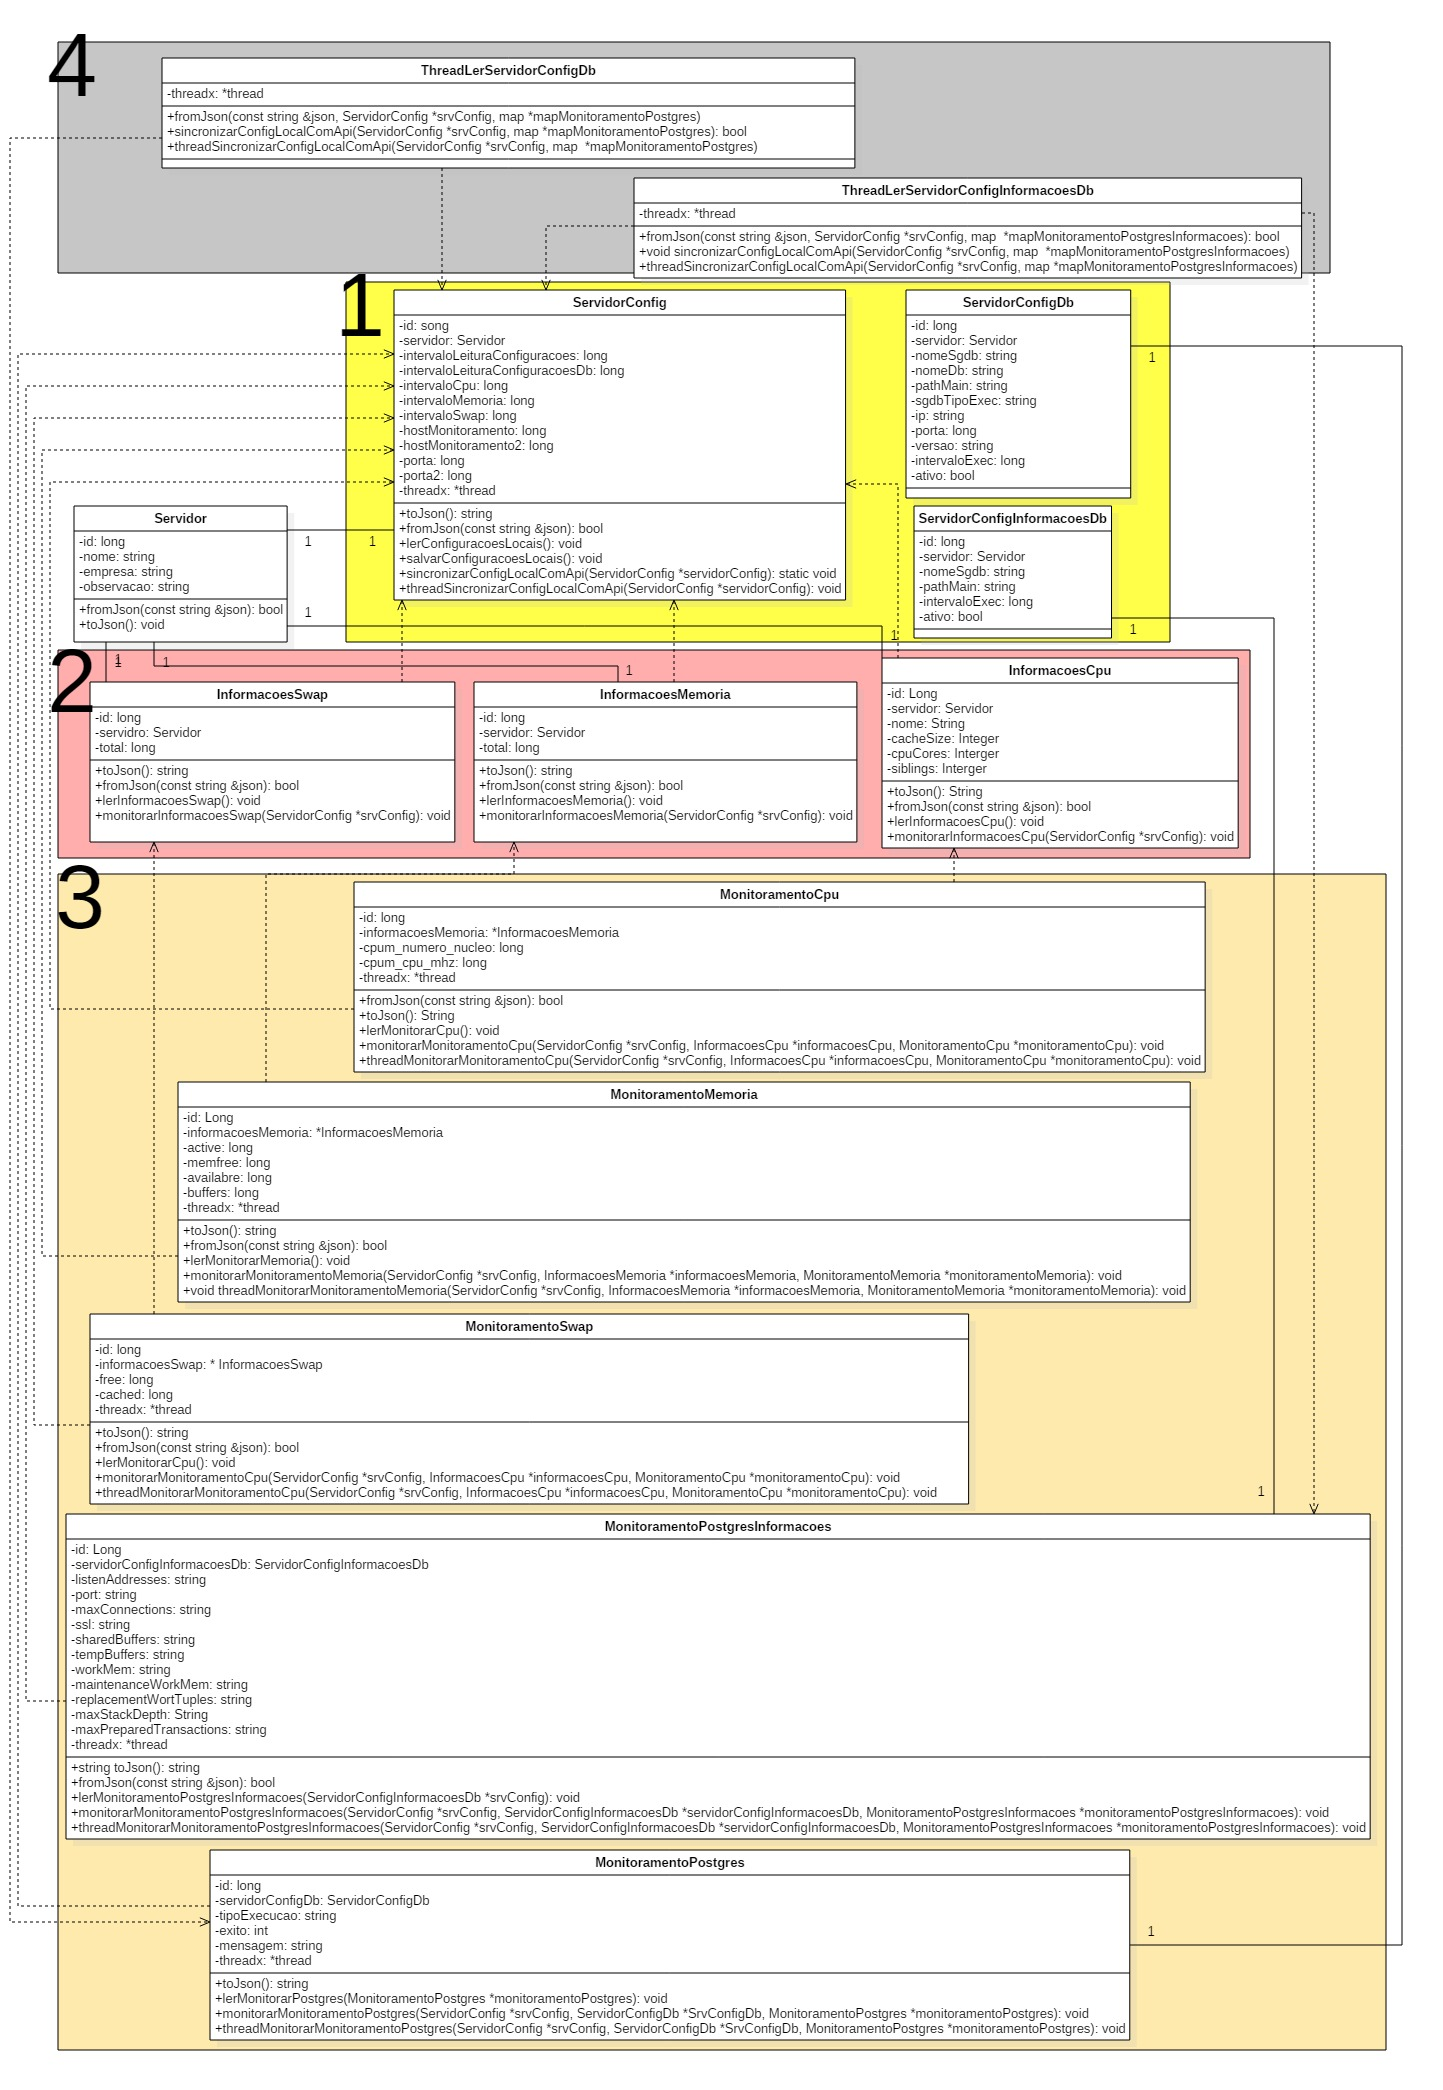
\includegraphics[width=1.0\textwidth]{figuras/Cli-Diagrama.jpg}
	\caption[Diagrama de classe do MonitoreWeb-Cli.]{Diagrama de classe do MonitoreWeb-Cli mostrando as relações entre as classes e dependências.}
	\label{Img:Cli-Diagrama}
\end{figure}


\subsection{Estrutura do Projeto}\label{}

O projeto é dividido em dois pacotes: o Entity, que contém as classes das entidades, descritas na \autoref{subsec:DiagramaDeClassesMonitorwebcli}; e o pacote Util, que contém as bibliotecas criadas neste projeto para atender a diversas finalidades, conforme descritas nas seguintes subseções. Além disso, contém a classe main.cpp, responsável por iniciar a aplicação. Essa classe é explicada na \autoref{subsec:executandoMonitorWeb-clie}.


\begin{figure}[H]
	\centering
	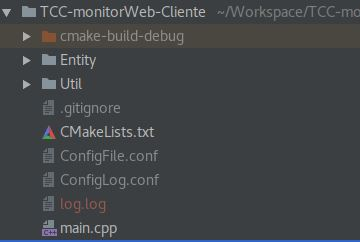
\includegraphics[width=0.5\textwidth]{figuras/pacotes-monitoreWeb-Cli.jpg}
	\caption[Pacotes da aplicação MonitoreWeb-Cli.]{Pacotes da aplicação MonitoreWeb-Cli.}
	\label{Img:Cli-Diagrama}
\end{figure}



\subsubsection{SystemLog}

Biblioteca para gerenciar os log que são mostrados na tela ou no arquivo log.log. Essa biblioteca realiza a leitura de suas configurações no arquivo configLog.conf. Esse arquivo foi explicado na \autoref{subsec:ConfiguracesMonitorWeb-CliConfigFile}.

\subsubsection{SystemData}

Biblioteca responsável por gerenciar data e hora da aplicação. Ela é utilizada pela SystemLog para registrar o instante de cada registro.

\subsubsection{ConfigFile}

Biblioteca responsável por realizar a leitura e escrita de arquivos com a estrutura "chave e valor" no HD. Essa biblioteca é utilizado por diversas classes na aplicação, entre ela esta a ServidorConfig que realiza a leitura do arquivo configFile.conf e depois a escrita. 

\subsubsection{Resource}

Biblioteca responsável por criar a requisição HTTP e realizar a comunicação com o MonitoreWeb-Api utilizando-se o protocolo TCP. Ele pode ser utilizado tanto para obter informações no servidor (GET) quanto para enviar requisições (POST). 

\subsection{Diagrama de Sequencia}\label{subsec:executandoMonitorWeb-clie}

Na \autoref{Img:MonitorWeb-Cli-DiagramaDeSequencia} mostra-se um diagrama de sequencia, continuado na  \autoref{Img:MonitorWeb-Cli-DiagramaDeSequencia2}. Esse diagrama possui quatro "linhas de vida"  representando, respectivamente, o servidor Linux, o MonitorWeb-Cli, o MonitorWeb-Api e o banco de dados.

Cabe observar que as setas com ponta fechada representam uma transação síncrona, as de ponta aberta representam transações assíncronas ou a criação de \textit{thread}, e as de pontas abertas e pontilhada representam um retorno.

Todos os métodos mostradas na \autoref{Img:MonitorWeb-Cli-DiagramaDeSequencia} e na \autoref{Img:MonitorWeb-Cli-DiagramaDeSequencia2} foram mostrados na \autoref{subsec:DiagramaDeClassesMonitorwebcli}. 

Na lista a seguir é descrito as relações entre cada uma das "linhas de vida" das aplicações.

\begin{itemize}
	\item Relação 1: assim que iniciada a aplicação, é chamado o método lerConfigLog para realizar a leitura das configurações do log, como pode ser visto na \autoref{subsubsec:ConfiguracesMonitorWeb-CliConfiglog}.
	
	\item Relação 2: o método lerConfiguracoesLocais realiza a leitura do arquivo lerConfigFile e configura o principal objeto da aplicação, o ServidorConfig. Mais detalhes sobre o arquivo pode ser visto na \autoref{subsubsec:ConfiguracesMonitorWeb-CliConfigfile}.
	
	\item Relação 3: neste momento uma \textit{thread} é criada deixando duas execuções em paralelo na aplicação. A nova \textit{thread} entrara em um \textit{loop} que ira durar até a aplicação ser encerada e a \textit{thread} antiga ira para a Relação 6.
	
	\item Relação 4 à 5: essa \textit{thread} tem a finalidade de atualizado o objeto ServidorConfig com os valores mais atuais do MonitorWeb-Api. Assim que ela é iniciada uma consulta (GET) é feita para o sistema servidor, que por sua vez solicita os valores para o banco de dados e devolve o resultado para o sistema cliente.
	
	\item Relação 6 e 11: essas relaçãos efetuam as leituras das informações do \textit{hardware} e enviam essas informações para o sistema servidor, que responde com um json contendo o objeto já persistido no banco de dados.
	
	\item Relação 12 à 20: nessas relações são criadas três novas \textit{threads} que se repetem até a aplicação ser encerada pelo usuário. Essas \textit{threads} são criadas para monitorarem CPU memória e \textit{swap}, elas realizam a leitura dos dados e enviam as informações para o sistema servidor realizar a persistência.
	
	\item Relação 21: é criado uma \textit{thread} para o monitoramento das informações do banco de dados.
	
	\item Relação 22 e 23: é realizada uma solicitado HTTP para o servidor, que por sua vez retorna um JSON contendo um vetor de objetos da classe MonitoramentoPostgresInformacoes. Esse vetor é percorrido e para cada objeto é criado uma \textit{thread}.
	
	\item Relação 24 e 25: é realizado leitura do arquivo de configurações do PostgreSQL (postgresql.conf), e seus valores são enviados para o servidor realizar a percistencia dos dados.
	
	\item Relação 26 e 27: é realizada uma solicitado HTTP para o servidor, que por sua vez retorna um JSON contendo um vetor de objetos da classe MonitoramentoPostgresDb. Esse vetor é percorrido e para cada objeto é criado uma \textit{thread}.
	
	\item Relação 28 e 30: é realizada as rotinas de \textit{backup} e \textit{vacuum}. Após o término, é enviada uma mensagem para o servidor informando se o procedimento foi nem sucedido ou não.
	
	\item loop: a \textit{thread} fica parada para que o sistema continue em execução.
	

\end{itemize}

\begin{figure}[H]
	\centering
	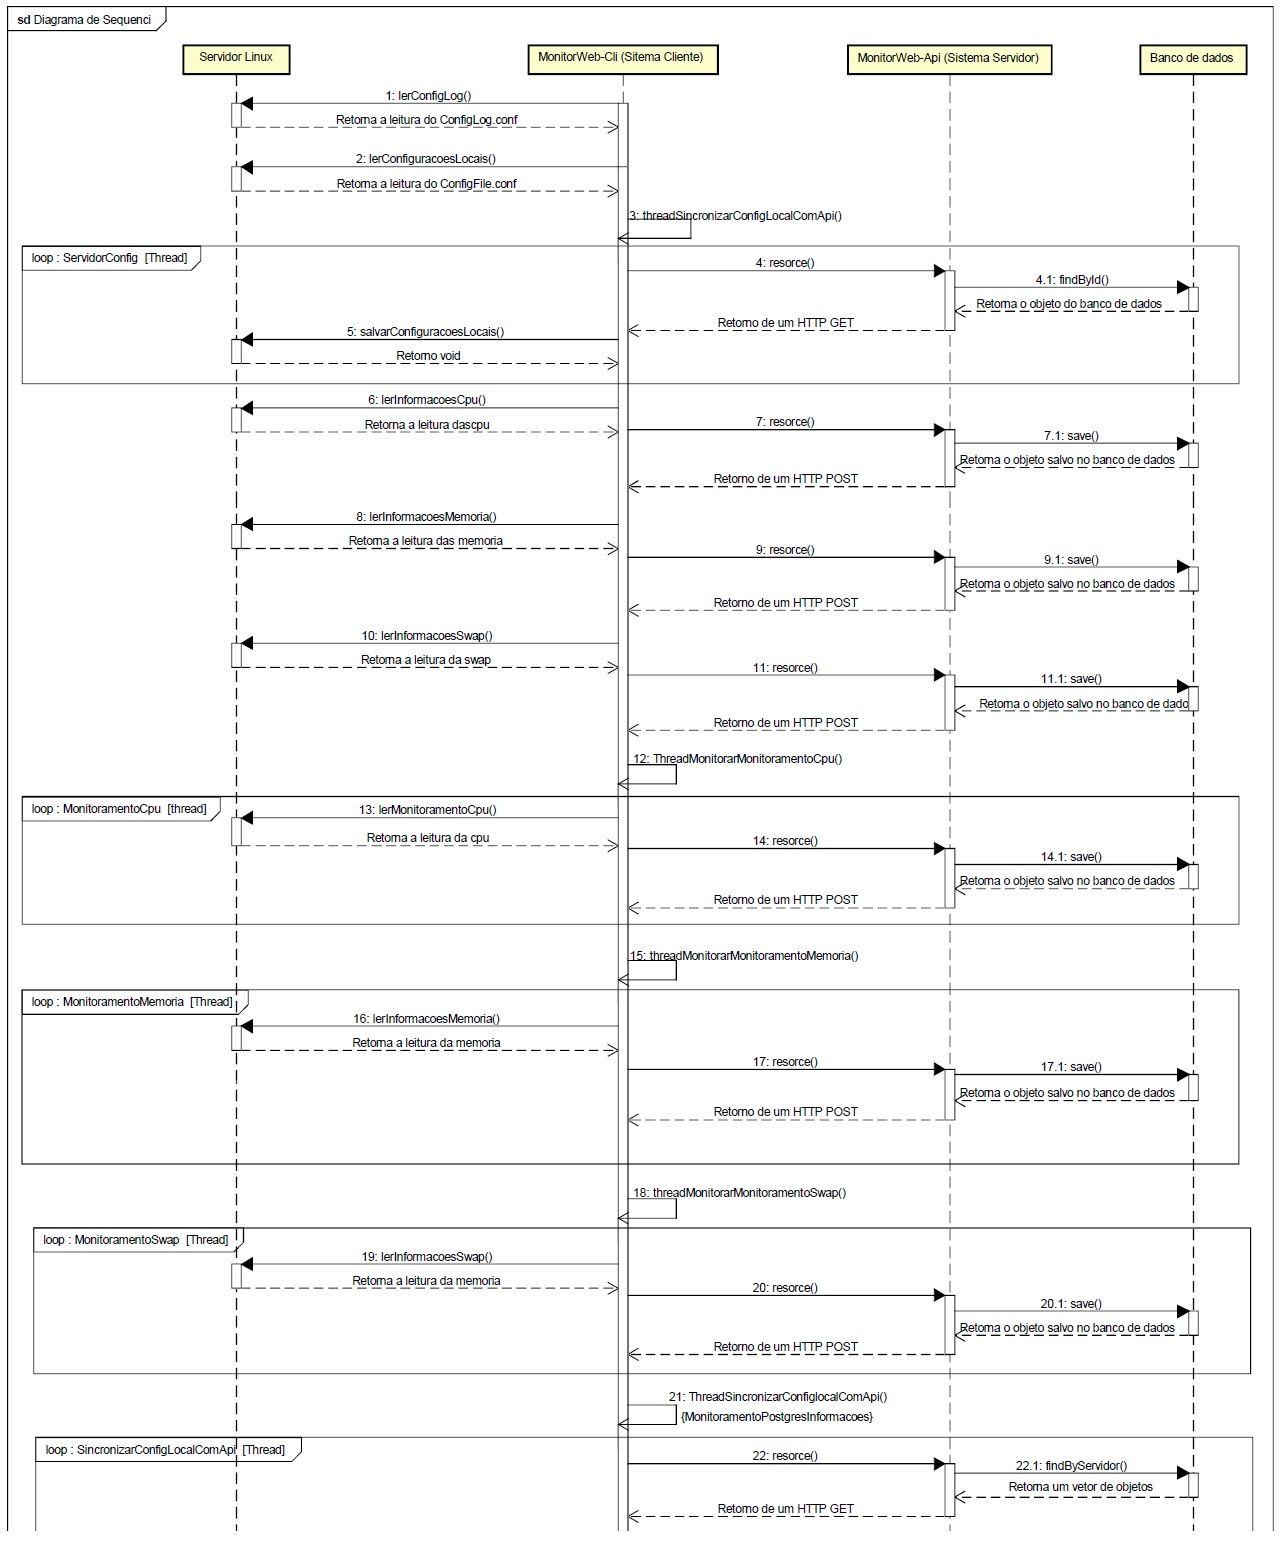
\includegraphics[width=1.0\textwidth]{figuras/diagramaSequencia1.jpg}
	\caption[Diagrama se sequencia da aplicação MonitorWeb-Cli parte 1.]{Diagrama se sequencia da aplicação MonitorWeb-Cli parte 1.}
	\label{Img:MonitorWeb-Cli-DiagramaDeSequencia}
\end{figure}

\begin{figure}[H]
	\centering
	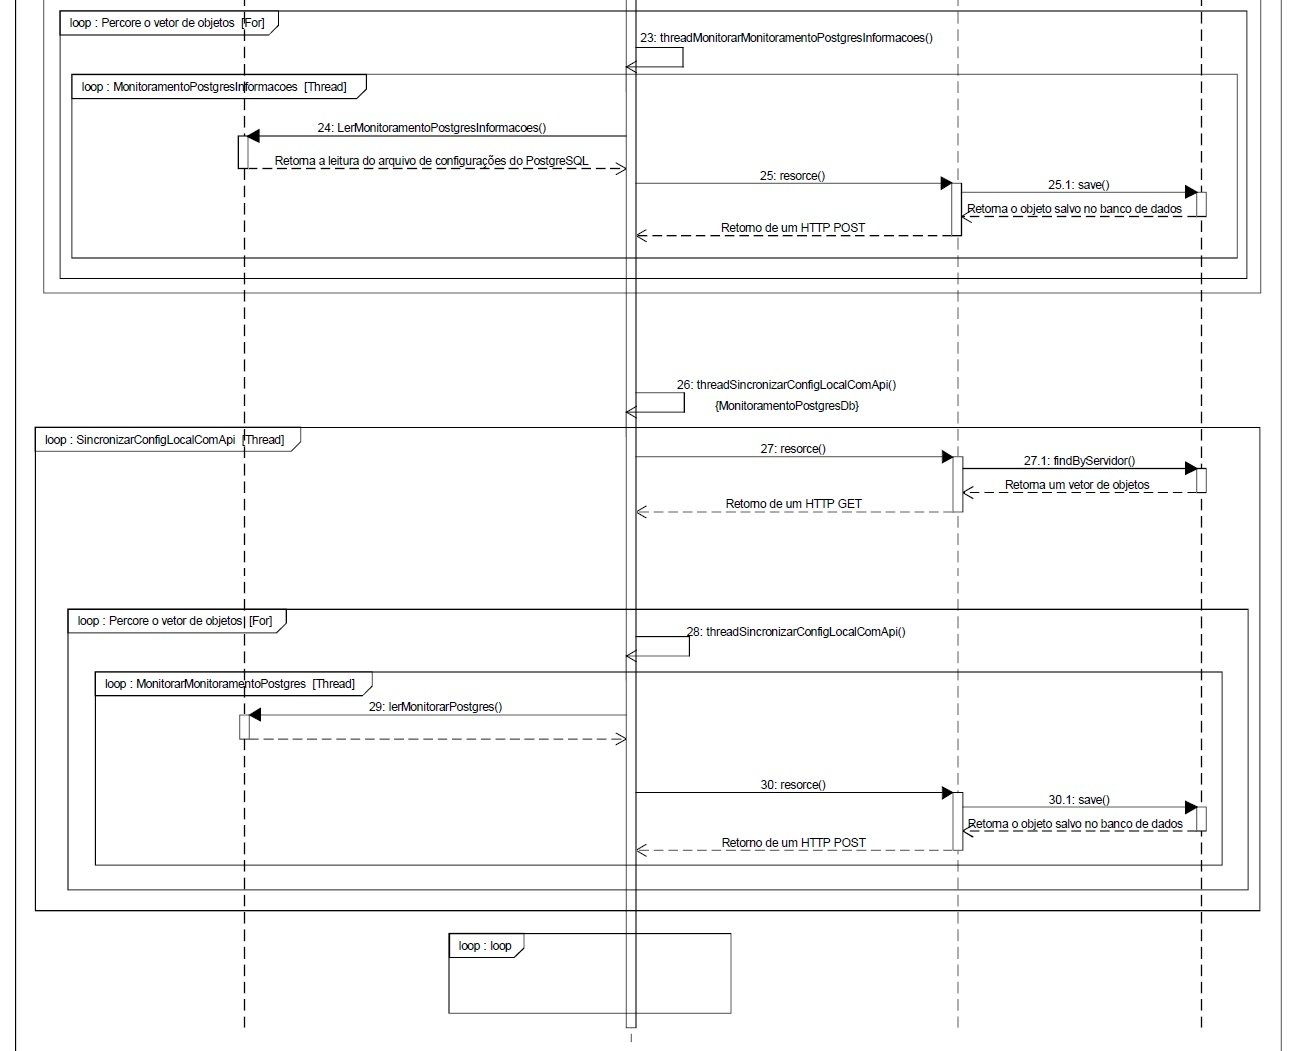
\includegraphics[width=1.0\textwidth]{figuras/diagramaSequencia2.jpg}
	\caption[Diagrama se sequencia da aplicação MonitorWeb-Cli parte 2.]{Diagrama se sequencia da aplicação MonitorWeb-Cli parte 2.}
	\label{Img:MonitorWeb-Cli-DiagramaDeSequencia2}
\end{figure}


